% STATUS: ACTIVE -- amplitude-writing single-parameter probe (2026-08-09).
%          Stage 1 = derivation only (this file's first two pages); the result
%          pages are appended after the 12-seed arms run.
%          p.1 derivation  the tie, the two Jacobians, the reading, the chain
%          p.2 figure      test_script/scratch/plot_formB_amp_prior_chain.m
%                          -> figures/formB_amp_prior_chain.png
% ======================================================
% Compile: xelatex formB_amp_bonly_probe.tex
% Path:    reference/eq17_analysis/derivation/formB_amp_bonly_probe.tex
% Truth:   calc_correction_functions (two-sphere perpendicular series)
% Scope:   this probe deliberately runs a writing that formB_ws_ref.tex S1
%          rules out; the scope limitation is stated on p.1 and the SSOT is
%          NOT modified.
% ======================================================

\documentclass[11pt,a4paper,fontset=none]{ctexart}

\usepackage[fleqn]{amsmath}
\usepackage{amssymb}
\setlength{\mathindent}{0pt}
\usepackage{geometry}
\geometry{margin=2.0cm}
\usepackage{graphicx}
\usepackage{booktabs}

\setlength{\parindent}{0pt}
\setlength{\parskip}{0.80em}
\linespread{1.08}

\begin{document}

\section*{The amplitude writing as a single-parameter probe}

The production law and the amplitude writing, both with the exponent pinned at
$p=1$ and the law origin pinned at the nominal contact $\bar{w}_s = 1$:
\begin{align*}
\text{Form B (length, production)}\quad
  \bar{a} &= 1 - \frac{b}{(\bar{w}-1) + b} \\
\text{Form C (amplitude, this probe)}\quad
  \bar{a} &= 1 - \frac{b}{\bar{w}}
\end{align*}

\textbf{Form C is Form B with the two states tied.} Setting $\bar{w}_s = b$ in
the production law with $p=1$,
\begin{equation*}
1 - \Bigl(1 + \frac{\bar{w}-b}{b}\Bigr)^{-1}
  = 1 - \frac{b}{\bar{w}} ,
\end{equation*}
identically. The probe therefore needs no new law: it opens a single free
scalar $\beta$ along the $(b,\bar{w}_s)$ diagonal of the existing controller.
By the chain rule along that diagonal, evaluated at the tied point,
\begin{equation*}
J_\beta = J_b + J_{w_s} = \frac{1}{\bar{w}^{2}} ,
\qquad
\frac{\partial\bar{a}}{\partial\beta}
  = \frac{\partial\bar{a}}{\partial b}
  + \frac{\partial\bar{a}}{\partial \bar{w}_s}
  = -\frac{1}{\bar{w}} ,
\end{equation*}
both exact. These are the closed forms already carried by
\texttt{formB\_amp\_functions.tex}.

\textbf{Why the probe exists.} The production Jacobian
$J_b = (g-b)/(g+b)^3$, $g = \bar{w}-1$, \emph{vanishes at} $g = b$, i.e.\
$\bar{w} = 1 + \hat{b} \approx 2.125$ ($h = 4.78\,\mu$m). The canonical
oscillation spans $h \in [4.5,\ 9.5]\,\mu$m, so the production arm crosses its
own $b$-channel null twice per cycle and sits $0.28\,\mu$m from it during the
final hold, where $|J_{w_s}/J_b| = 2b/|g-b| = 18$. The tied Jacobian
$1/\bar{w}^{2}$ is strictly positive with no null anywhere. The probe asks
whether that difference is what has kept $\hat{b}$ from moving.

\textbf{Scope limitation against the SSOT.}
\texttt{formB\_ws\_ref.tex} S1 rules the amplitude writing out on two grounds:
fitted with a free origin it returns $\bar{w}_s = -0.063$, not a surface
position; and it drags fractional powers and logarithms into every Jacobian.
Neither applies here --- the origin is pinned at $1$ and the exponent at $1$,
so the Jacobians above are rational and the origin is not a fitted quantity.
The SSOT stands; this file records only the scoped exception.

\textbf{What the tie costs, stated before the run.} At the same $b$ the
production law is evaluated at $g = \bar{w}-1$ and the tied law at
$\bar{w}$: these are two different model classes, not a reparametrisation of
one filter. On the canonical envelope the anchored-seed shape floor is
$0.00284$ for Form B against $0.03724$ for Form C, a factor $13.1$; at the
final hold ($\bar{w}=2$) the anchored gains are $-0.01\,\%$ and $-7.04\,\%$
against the truth. A worse gain error in the amplitude arm is therefore the
\emph{expected} outcome and is not evidence against the probe; the criteria
are the $b$-channel ones.

\subsection*{The prior width, by the six-step chain}

Steps follow \texttt{reference/shared/param\_prior\_rules.md}.

\textbf{(2) Seed from an analytic anchor.} The far-field truth deficit is
$1-\bar{a} \simeq (9/8)/\bar{w}$, and the amplitude writing's deficit is
$b\,\bar{w}^{-p}$, so \emph{one} limit pins both constants: $b_0 = 9/8$,
$p_0 = 1$. The ignorance source of the error is zero.

\textbf{(3) The reading.} Taking logarithms of the deficit,
\begin{equation*}
\ln(1-\bar{a}) = \ln b - p \ln \bar{w} ,
\end{equation*}
so $b$ is the log-log \emph{intercept} and $p$ is the slope. With $p$ pinned
the intercept is read directly against the truth --- unlike the production
writing, where $b$ sits inside a bracket and the level-versus-slope choice
needs the argument of S10:
\begin{equation*}
b_{\mathrm{eff},\text{C}}(\bar{w}) = \bar{w}\,(1-\bar{a}_{\mathrm{true}})
  = \bar{w}\,\frac{c-1}{c} ,
\qquad
b_{\mathrm{eff},\text{B}}(\bar{w}) = (c-1)(\bar{w}-1) .
\end{equation*}
Both run from $1$ at contact to $9/8$ in the far field: each traverses exactly
the $12.5\,\%$ anchor tension, and the global $\sup$ \emph{is} that tension
($0.1250$ and $0.1244$; the difference is the sweep starting at
$\bar{w}=1.001$).

\textbf{(5)--(6) The $\sup$ domain and the width.} On the canonical envelope
$[1.90,\ 22.3]$ (commanded trough $2.0$ less the derived margin $0.1$;
start height plus $1$),
\begin{equation*}
\sqrt{P_{\beta\beta}[0]} = \sup_{\text{envelope}}
  \bigl|b_{\mathrm{eff},\text{C}} - 9/8\bigr| = 0.0708 ,
\qquad
\text{(production: } 0.0157\text{)} .
\end{equation*}

Two independent criteria select the envelope over the global fallback
$0.125$. Rule 3 (\emph{just enough, not more}): the value the truth demands at
the final hold is $b_{\mathrm{eff},\text{C}}(2) = 1.0588$, a travel of
$0.94\,\sigma$ against $0.0708$ but only $0.53\,\sigma$ against $0.125$ ---
$1.9\times$ over-wide, the regime the 2026-08-01 revision exists to remove.
And the $P[0]$ budget: at the predicted $\sim\!90\,\%$ contraction the
realised ratio $(\Delta\beta)^2/(P[0]-P[\infty])$ is $0.97$ against a limit of
$1$, versus $0.31$ for the global width. The envelope prior is TIGHT by
construction, i.e.\ $\sup|\theta_{\mathrm{eff}}-\theta_0| \div \sqrt{P[0]}
= 1.00\times$, the same honesty status the production widths carry.

The shape floor on the same envelope, which funds $P_{\bar{a}\bar{a}}[0]$, is
\begin{equation*}
\text{floor}_{a,\text{C}}
 = \sup_{\text{envelope}}\Bigl|1-\tfrac{9/8}{\bar{w}} - \tfrac{1}{c}\Bigr|
 = 0.03724
 \;\equiv\; \sup_{\text{envelope}}
   \frac{|b_{\mathrm{eff},\text{C}} - 9/8|}{\bar{w}} ,
\end{equation*}
the identity holding pointwise and used as the driver's self-check (residual
$1.4\times10^{-17}$).

\subsection*{Declared boundary sensitivity}

$b_{\mathrm{eff},\text{C}}$ is strictly monotone, so its $\sup$ sits on the
envelope \emph{floor}; $b_{\mathrm{eff},\text{B}}$ is not, and its $\sup$ sits
at the interior point $\bar{w} \approx 4.28$. Refitting the floor:

\begin{center}
\begin{tabular}{lccc}
\toprule
envelope floor & $1.90$ & $1.95$ & $2.00$ \\
\midrule
$\sqrt{P[0]}$, Form B (production) & $0.0157$ & $0.0157$ & $0.0157$ \\
$\sqrt{P[0]}$, Form C (this probe) & $0.0708$ & $0.0685$ & $0.0663$ \\
\bottomrule
\end{tabular}
\end{center}

The production comment that the envelope margin is ``insensitive by design''
is therefore true only for the length writing. For the amplitude writing the
margin's provenance is load-bearing and is restated here: $0.1$ is the
measured true-trough undershoot $0.033\,R$ plus position measurement noise
$\sim\!0.05\,R$, rounded up. A $0.05\,R$ error in that margin moves the
declared prior by $6.4\,\%$. This is a declared sensitivity, not a tuning
knob.

\clearpage

\begin{center}
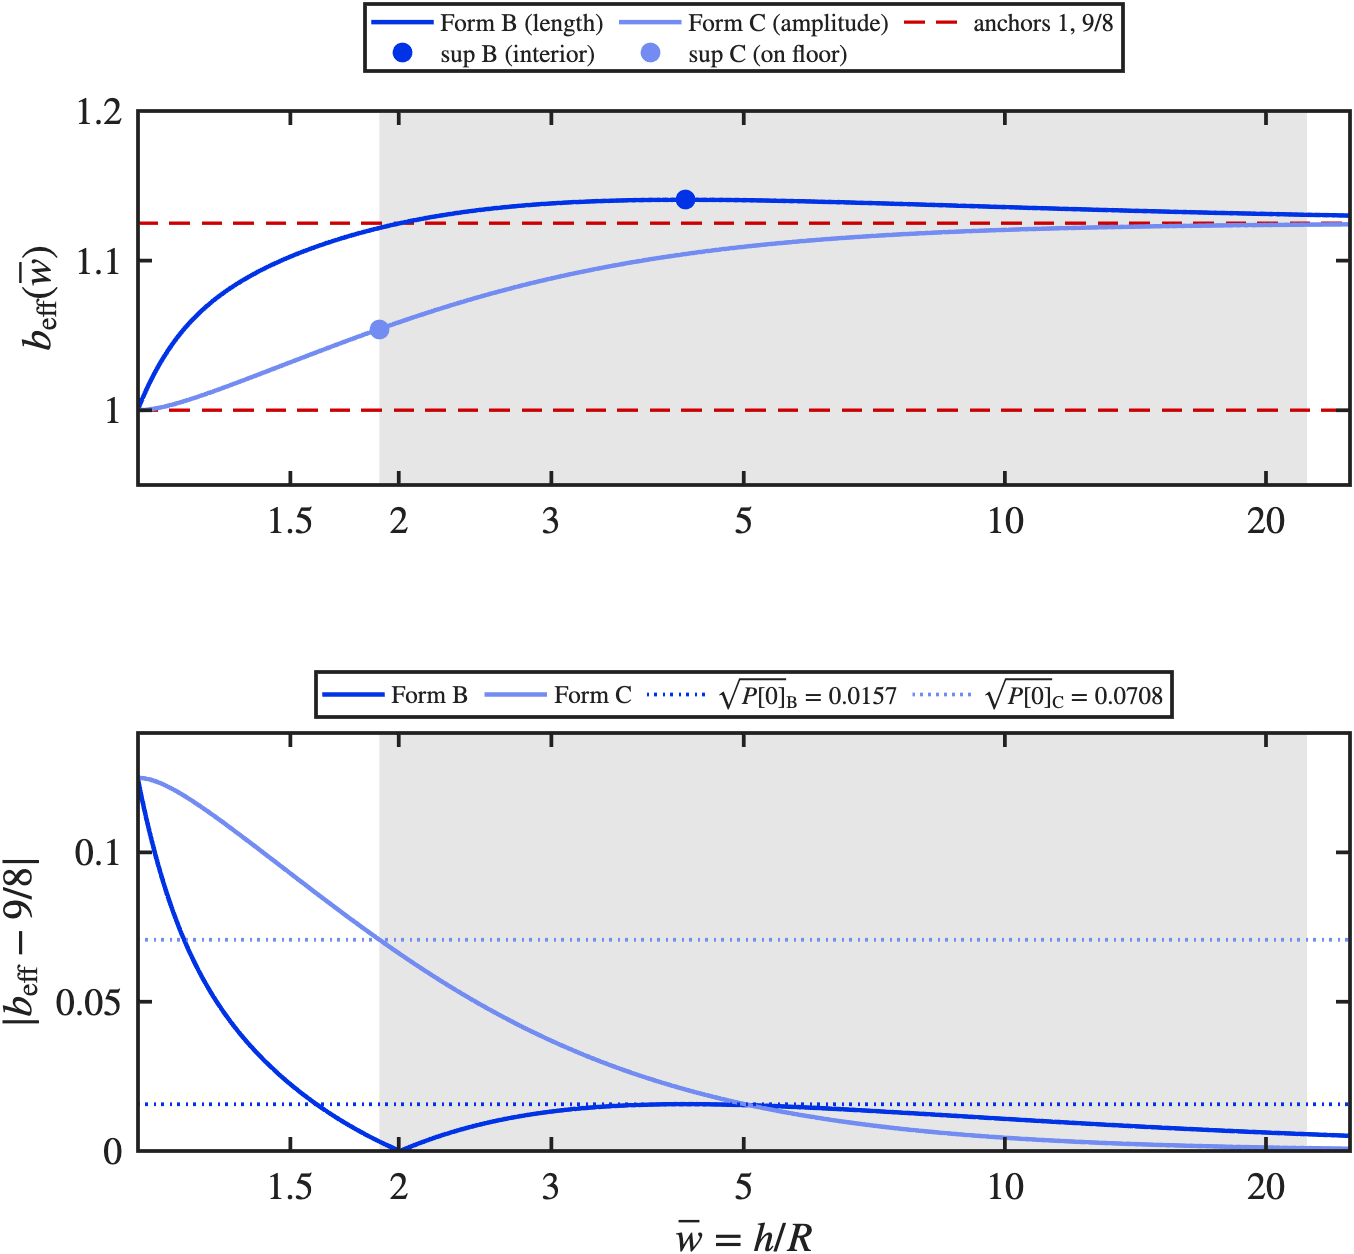
\includegraphics[width=0.92\linewidth]{figures/formB_amp_prior_chain.png}

Step 3 of the $P[0]$ chain for both writings, with nothing fitted: each curve
is the constant its own law demands of the published truth at each height.
Top --- both readings travel from the contact anchor $1$ to the far-field
anchor $9/8$, so the global $\sup$ is the $12.5\,\%$ anchor tension in either
writing; the shaded band is the canonical envelope $[1.90,\ 22.3]$ and the
filled circles mark where each $\sup$ is attained. Bottom --- the same
quantity as a prior budget. The production reading is non-monotone, crosses
its own anchor near $\bar{w} \approx 2.5$ and peaks in the interior, which is
why its width $0.0157$ is identical for envelope floors $1.90/1.95/2.00$. The
amplitude reading is monotone, so its width $0.0708$ is attained on the floor
itself and inherits the margin's provenance directly ($0.0708/0.0685/0.0663$
across the same three floors, a $6.4\,\%$ spread). The $4.5\times$ ratio
between the two widths is not a modelling choice --- it is what the two
writings honestly cost on the heights this scenario visits, and it is half of
why the amplitude arm's $b$ channel is expected to be live where the
production one is not (the other half being the Jacobian null at
$\bar{w} = 1+\hat{b}$, which the amplitude writing does not have).
\end{center}

\clearpage

\section*{Result: the arm ladder}

Plant = the real plane wall; the controller knows nothing about it and every
seed is the far-field anchor. Twelve seeds, one scenario, identical noise
realisation per seed across arms. Each rung changes exactly one thing, so the
three effects add. Structural acceptance (\texttt{verify\_formB\_amp\_tie}:
default bit-identity, the closed-form fold to $9\times10^{-16}$, the tie
verified inside the shipped controller to $1.3\times10^{-15}$, finite
differences, the pole guard, covariance health) passed before any number here
was read.

\begin{center}
\begin{tabular}{llccccc}
\toprule
 & arm & $\hat{\beta}$ final & $\sqrt{P}$ shrink & budget & desc \% & hold \% \\
\midrule
A0 & \texttt{len\_prod} \small(b,p free) & $1.1247 \pm 0.0035$ & $2.1\%$  & $1.15$ & $1.55$ & $-0.39$ \\
A1 & \texttt{len\_bonly}                 & $1.1246 \pm 0.0054$ & $3.2\%$  & $1.74$ & $1.10$ & $-0.47$ \\
A2 & \texttt{len\_wide} \small(prior $\times 4.5$) & $1.1207 \pm 0.0500$ & $35.0\%$ & $0.81$ & $2.10$ & $-0.30$ \\
A3 & \texttt{len\_ws98} \small(origin $9/8$) & $1.0923 \pm 0.0312$ & $14.6\%$ & $1.47$ & $6.93$ & $-4.98$ \\
A4 & \texttt{amp} \small(the tie)        & $1.0821 \pm 0.0340$ & $38.1\%$ & $1.00$ & $6.60$ & $-3.08$ \\
\bottomrule
\end{tabular}
\end{center}

\textbf{Travel decomposition} (mean over 12 seeds, units of $R$):
\begin{center}
\begin{tabular}{lrr}
\toprule
A1 \ \texttt{len\_bonly}, production prior & $-0.00037$ & \\
$+$ prior width $0.0157 \to 0.0708$        & $-0.00396$ & (A1 $\to$ A2) \\
$+$ law origin $1 \to 9/8$                 & $-0.02834$ & (A2 $\to$ A3) \\
$+$ Jacobian fold $J_b \to J_b + J_{w_s}$  & $-0.01020$ & (A3 $\to$ A4) \\
\midrule
$=$ A4 \ \texttt{amp}                      & $-0.04287$ & \\
\bottomrule
\end{tabular}
\end{center}

Three readings, in order of how much they change the mainline.

\textbf{(i) Widening the prior alone buys essentially nothing.} A2 opens the
$b$ prior by $4.5\times$ and $\hat{b}$ still does not move ($-0.06\,\sigma$,
$9\,\%$ of the total travel) --- yet its variance drops $35\,\%$, almost as
much as the tied arm's $38\,\%$. \emph{Variance reduction and travel are
different things.} The length writing's $b$ channel does carry information;
it has nothing to say, because on this envelope the anchored $b$ is already
what the truth demands to within $0.0157$. On the 2026-08-06 arm the truth was
a constructed curve $63.5$ widths away and the prior was the binding
constraint; with the real plane wall it is not.

\textbf{(ii) The Jacobian fold is measurable and one-directional.} A3 and A4
share the law at $t=0$, the origin, the prior and the seed noise; they differ
only by $J_b \to J_b + J_{w_s}$. The fold adds $33\,\%$ more travel
($-0.0429$ vs $-0.0312$), $2.6\times$ more variance reduction
($38.1\,\%$ vs $14.6\,\%$), and cuts the residual hold error from
$-4.98\,\%$ to $-3.08\,\%$. Along the real trajectory the tied Jacobian is
$+0.25$ throughout the final hold where the production one is $-0.013$ --- a
factor $19$, at the height where the gain matters most and where the
production $J_b$ has changed sign.

\textbf{(iii) Where $\hat{\beta}$ lands was predicted correctly.}
Mean $1.0821$ against the pre-registered information-weighted
$\langle b_{\mathrm{eff}}\rangle = 1.0833$; $t = -4.36$ ($df$ 11) against the
``did not move'' hypothesis. The estimate does \emph{not} reach the envelope
minimax $1.0651$ or the trough-exact $1.0588$, exactly as the derivation
predicted: the prior width is set by the trough, which is the least
informative point on the trajectory, while the information sits in the
high-velocity descent. Consistency: $\mathrm{corr}(\hat{\beta},\ \text{hold
error}) = -0.80$, the sign the law requires; the traversal budget averages
$1.003$ against a limit of $1$, i.e.\ the arm consumes exactly the prior it
declared. Honesty: spread over seeds $\div$ claimed final $\sigma$ $= 0.78$.
One genuine outlier, seed 11 ($\hat{\beta} = 0.992$, hold $+5.3\,\%$, the only
positive one); it is an outlier in A3 as well, so it belongs to that noise
realisation and not to the writing. Excluding it the mean is $1.0903$ with
spread $0.0199$.

\textbf{What this does not license.} As a candidate production law the
amplitude writing fails on accuracy, as stated before the run: descent
$6.60\,\%$ and hold $-3.08\,\%$ against production's $1.55\,\%$ and
$-0.39\,\%$. Most of its travel is repairing a $8.4\,\%$ seed model error it
inflicted on itself by moving the law's zero-gain point to
$\bar{w} = \beta$. Its final absolute uncertainty is also worse
($\sqrt{P} = 0.0438$ vs the length arm's $0.0152$), because the length
writing's prior is tighter --- and it is tighter because that writing genuinely
fits the truth better on the heights this scenario visits. The
\texttt{formB\_ws\_ref} S1 ruling stands.

\textbf{What it does settle.} The production arm's $\hat{b}$ standing still is
\emph{correct behaviour, not a defect}: A2 shows that releasing the prior does
not move it, and A4 shows that the same filter moves $\hat{\beta}$ by
$-0.61\,\sigma$ reproducibly once there is something to learn. The b-channel
weakness diagnosed from the Jacobian null is real and worth $33\,\%$ of the
travel, but it is not what has been holding the mainline back.

\clearpage

\begin{center}
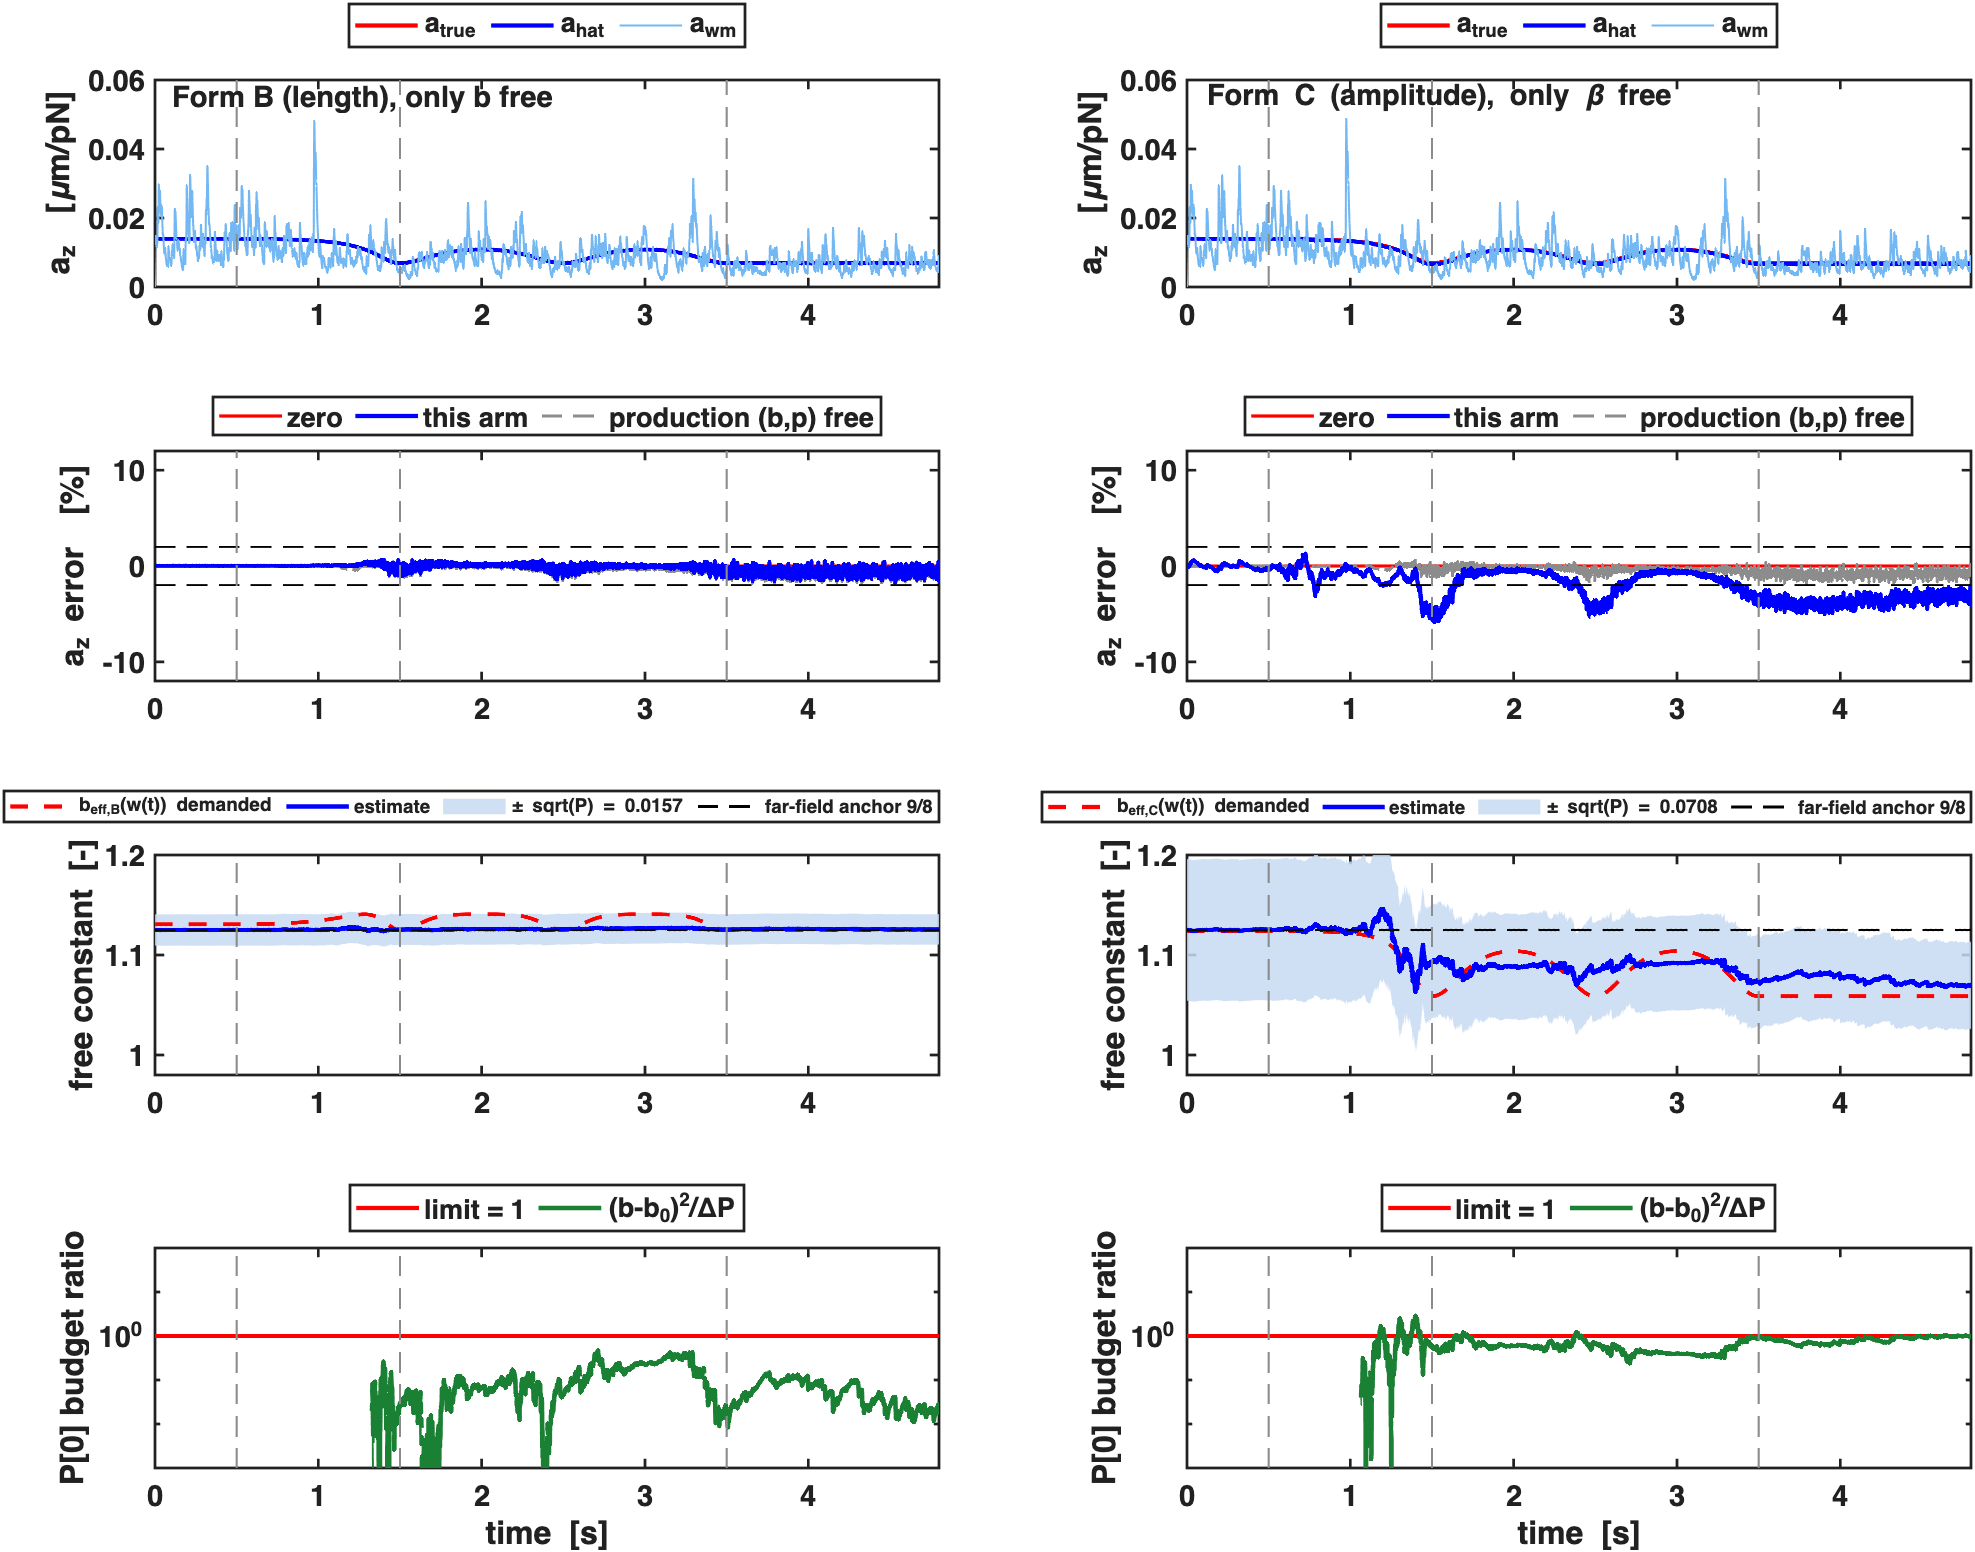
\includegraphics[width=0.98\linewidth]{figures/formB_bonly_BvsC_seed7.png}

Seed 7, both writings, only the shape constant free. Left the production
length writing, right the tie. Row 3 is the whole story: the length arm's
estimate sits on the anchor and the red dashed curve --- the constant the
truth demands at the height the particle is at --- sits on top of it, so there
is nothing to correct. The amplitude arm starts on the same anchor, walks down
through the descent and then tracks its own demanded curve. Row 4 shows the
traversal consuming the declared prior (ratio $\to 1$) rather than exceeding
it. Row 2 is the price: the amplitude arm runs at $-3$ to $-6\,\%$ where the
production reference (grey) sits inside $\pm 1\,\%$. Note also that the
amplitude arm's error is largest in the oscillation troughs and recovers at
the peaks --- the signature of a one-parameter family whose single constant
cannot be right at two heights at once.
\end{center}

\clearpage

\begin{center}
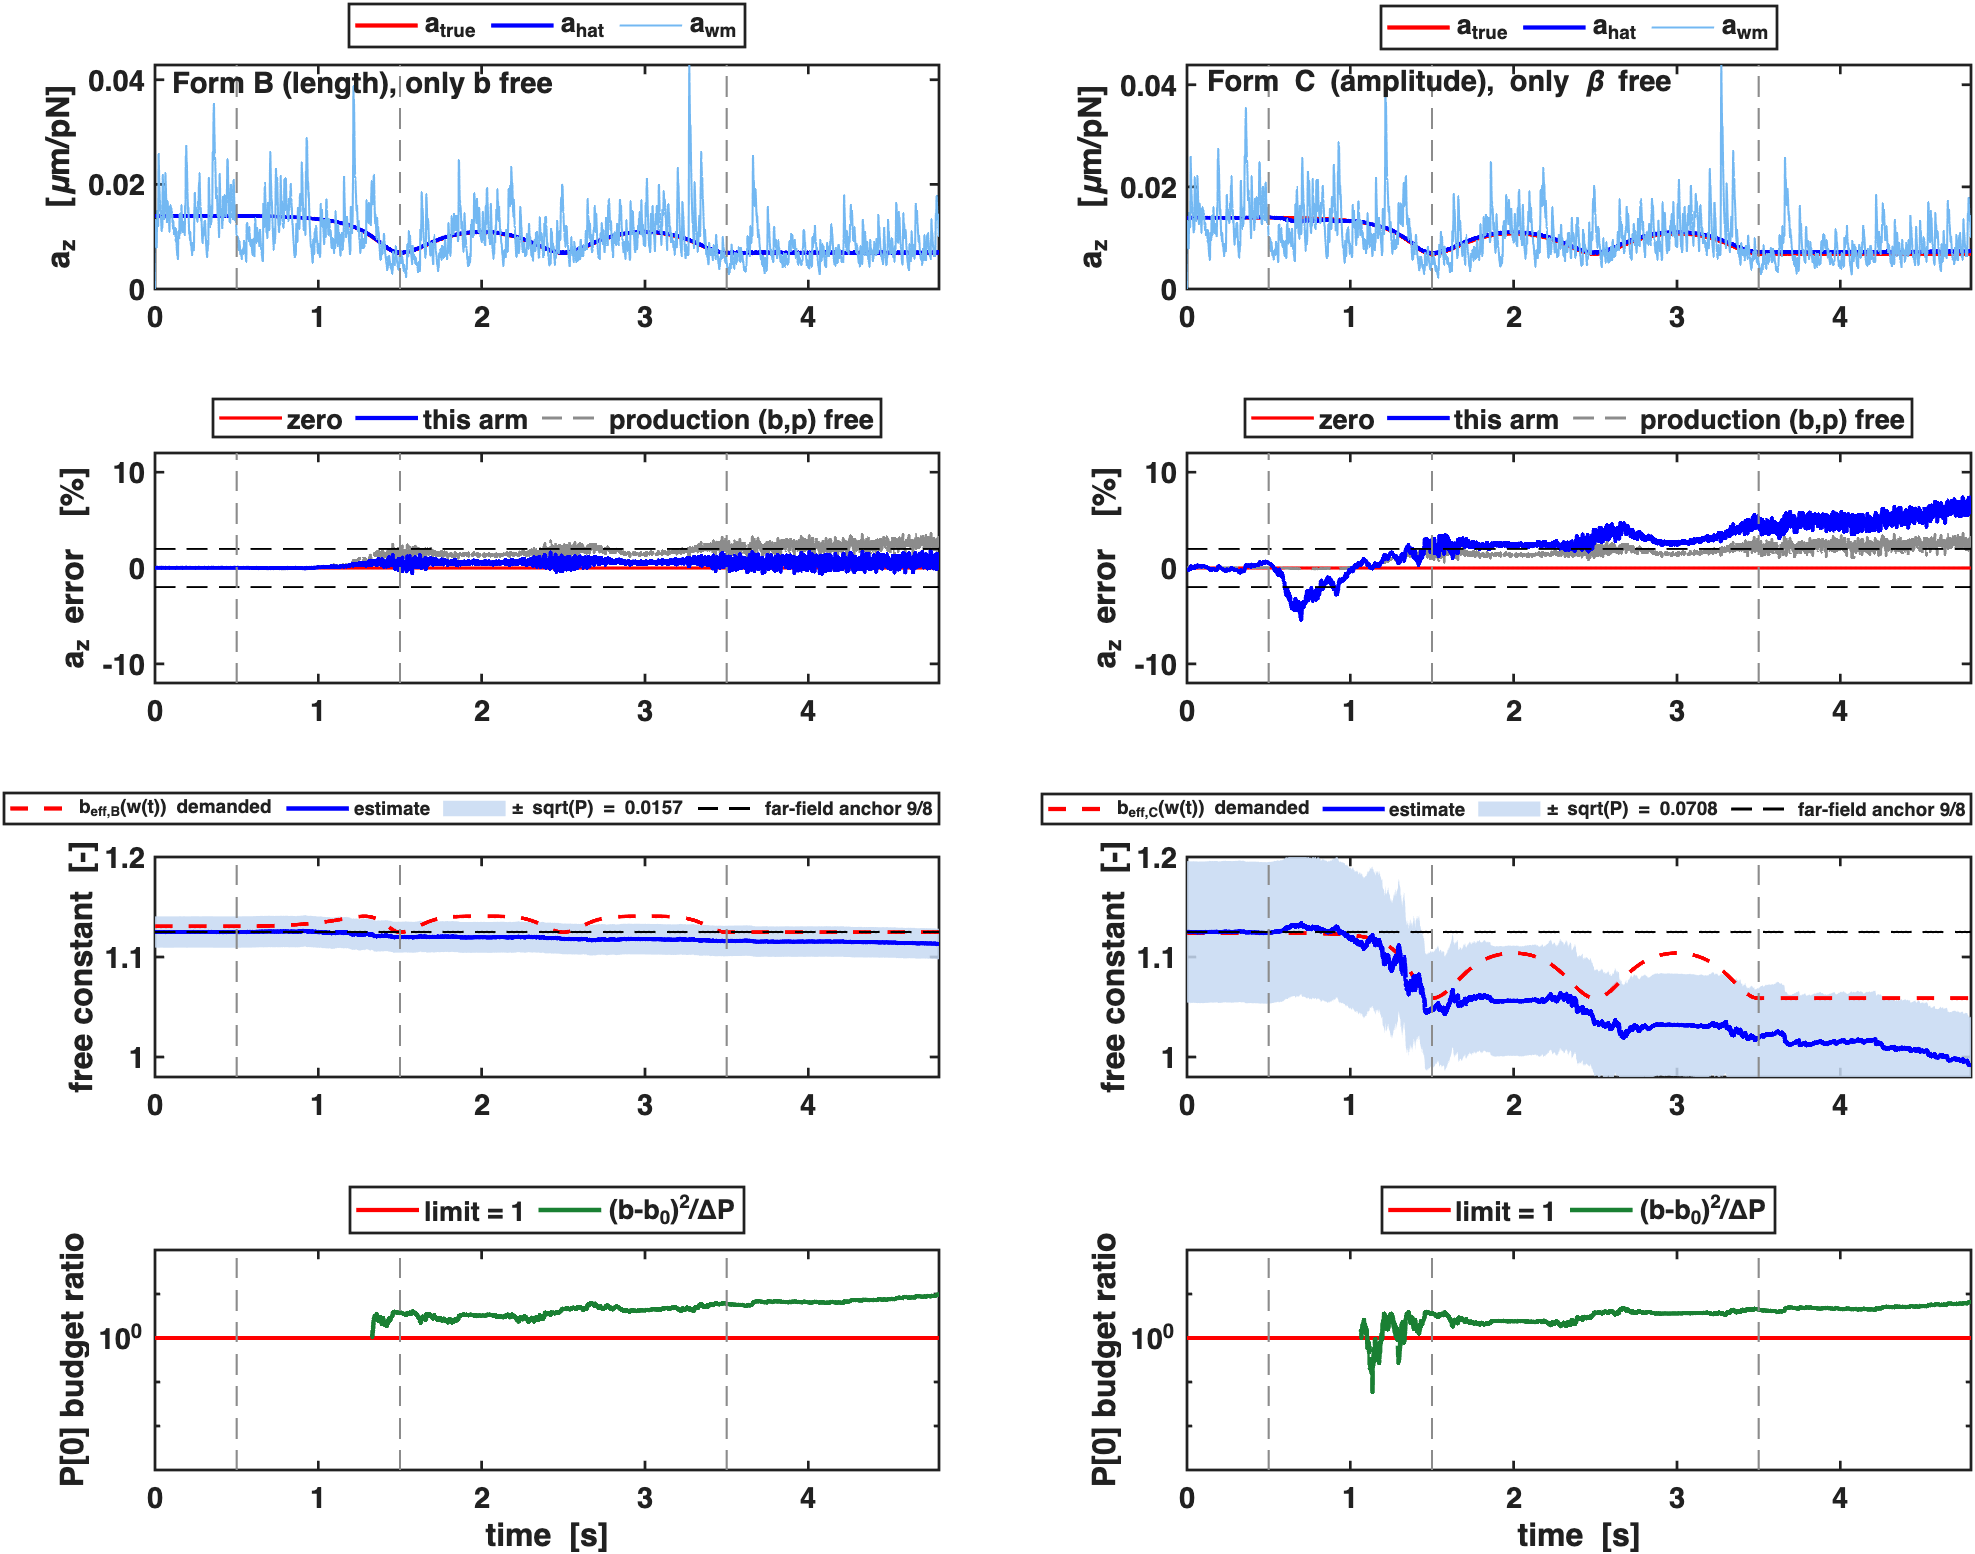
\includegraphics[width=0.98\linewidth]{figures/formB_bonly_BvsC_seed11.png}

Seed 11, the outlier, shown rather than dropped. Here $\hat{\beta}$ overshoots
to $0.992$ --- past every pre-registered target --- and the hold error goes
$+5.3\,\%$, the only positive one in the set. The same seed is the extreme of
the A3 arm too ($1.0151$), so this is a property of that noise realisation and
not of the writing: a run whose descent innovations happen to push the
constant too far, with nothing downstream able to pull it back because
$Q_{\beta\beta} = 0$ means the filter's confidence only ever grows. This is
the failure mode a single free constant with a hard zero process noise has,
and it is the reason the spread over seeds --- not the single-run number --- is
the reproducibility statistic.
\end{center}

\clearpage

\begin{center}
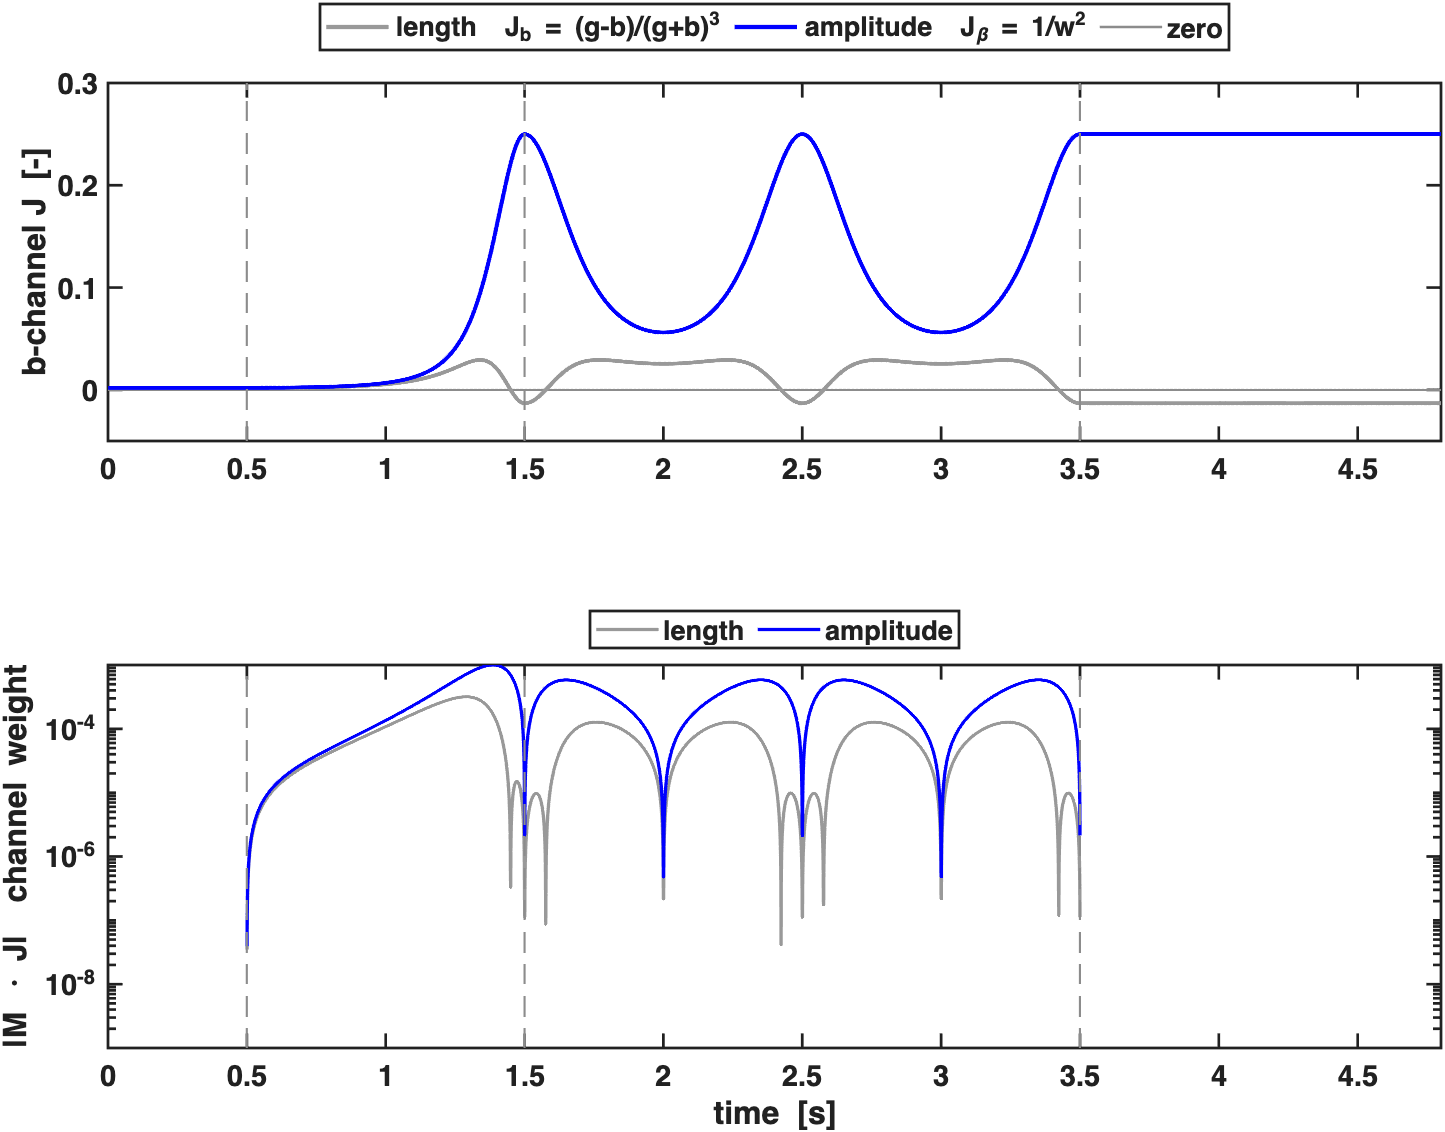
\includegraphics[width=0.85\linewidth]{figures/formB_amp_jacobian_live.png}

The $b$-channel Jacobian along the real trajectory (seed 7, evaluated at the
estimate the controller actually used). Top --- the production $J_b$ (grey)
sits near zero, dips \emph{negative} at every oscillation trough and stays
negative through the entire final hold; the tied $J_\beta = 1/\bar{w}^2$
(blue) peaks at $0.25$ at each trough and holds there, a factor $19$ at the
height where the gain matters most. Five sign changes after the initial hold.
Bottom --- the same quantity weighted by the commanded motion it enters with,
$|M \cdot J|$, on a log axis: the grey trace carries \emph{extra} nulls that
the blue one does not, one pair per cycle, and those are the Jacobian zeros,
distinct from the trajectory turning points where both traces null. This is
the offline page-5 prediction realised in closed loop.
\end{center}

\clearpage

\begin{center}
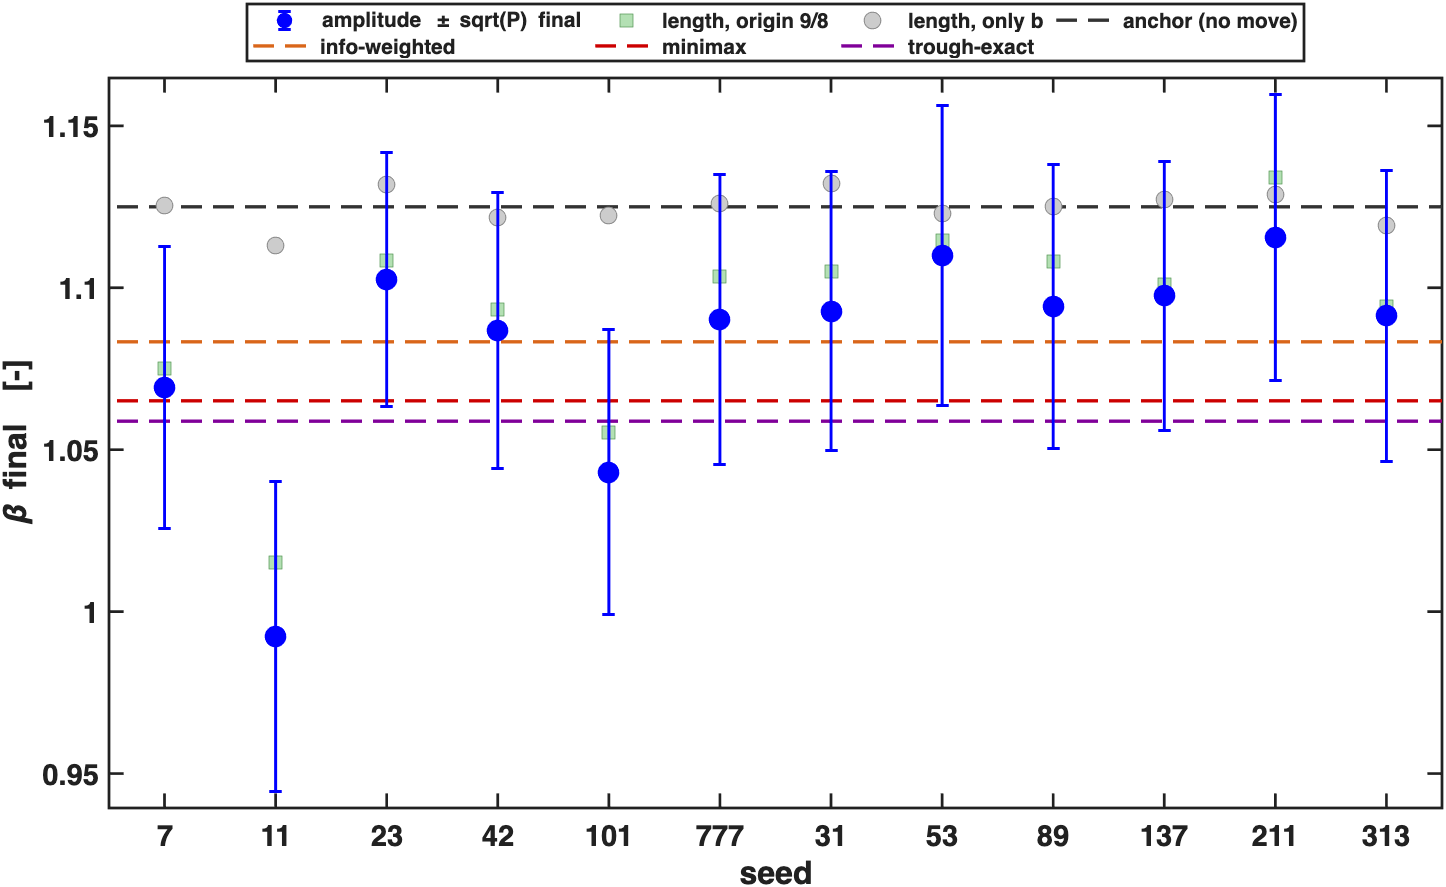
\includegraphics[width=0.85\linewidth]{figures/formB_amp_bhat_landing.png}

Final constant per seed against the four pre-registered landing hypotheses.
Grey circles: the length writing with only $b$ free --- pinned on the anchor,
spread $0.0054$, nothing learned. Green squares: the same writing with its
origin declared at $9/8$ (the fold negative control). Blue with error bars:
the tie, showing its own claimed final $\sqrt{P}$. The blue mean $1.0821$
lands on the information-weighted prediction $1.0833$ and clears the
``did not move'' line at $t = -4.36$; it does not reach the minimax or
trough-exact lines, which is what the derivation said would happen because the
prior is sized by the trough while the information sits in the descent.
Eleven of twelve seeds move monotonically downward; seed 11 overshoots.
\end{center}

\end{document}
